O método dos Elementos Finitos (MEF) foi criado como uma técnica
numérica com o intuito de encontrar soluções para os
problemas de valor de contorno para equações diferenciais
parciais. O FEM baseia-se em subdividir o domínio em pequenos
subdomínios nos quais são conhecidos como elementos e aplicar
a formulação variacional . 


O Método dos Elementos Finitos (MEF) é um método numérico
que consiste em encontrar soluções para as equações diferenciais 
parciais em problemas de valores de contorno. 

Segundo a Organização Mundial de Saúde (OMS) \cite{oms},
as doenças cardiovasculares são as principais
causas de óbitos no mundo. Cerca de 40\% dessas
mortes são ocasionadas por doenças na artéria
coronária (DAC). 

\medskip
Em 1964, \cite{dotter1964} introduz uma nova técnica para o tratamento
da artéria femoral obstruída devido a aterosclerose. Esta técnica é
conhecida como \textit{angioplastia transluminal percutânea} e consiste num
procedimento simples e minimamente invasivo, possibilitando a execução por qualquer 
médico familiarizado com a cateterização vascular. Tal procedimento se apresentou 
aplicável a outras artérias, inclusive a artéria coronária.

\medskip
Em 1979, \cite{gruntzig1979} realiza a técnica transluminal percutânea na artéria
coronária utilizando um cateter com balão inflável com o intuito de dilatar o local
com esterose. O procedimento foi realizado em 50 pacientes durante 18 meses e
apresentou-se resultados satisfatórios principalmente com pacientes com apenas
uma única artéria com esterose. Tal procedimento fica conhecido como \textit{Angioplastia Coronária
Transluminal Percutânea} (PTCA). 

\medskip
Embora o PTCA utilizando um balão inflável tenha apresentado resultados satisfatórios,
com o passar o tempo a artéria apresentava reestenose. Em 1987, \cite{sigwart1987}
apresenta o resultado da implantação de uma prótese constituida de uma malha de aço 
inoxidável auto-expansível nas artérias femoral e coronárias de 25 pacientes que apresentavam 
casos de reestenose. Embora a reestenose continuar presente, a prótese se mostrou uma
maneira interessante para a resolução da reestenose. Esta prótese recebeu o nome de \textit{stent}.

\medskip
Em 1994, \cite{serruys1994} apresenta uma comparação entre os procedimentos PTCA 
utilizando um balão inflável e a implantação do stent. Foram analisados 520 pacientes,
onde 262 pacientes com stents implantados e 258 pacientes somente com o procedimento do
balão inflável. Os resultados clínicos e angiográficos se apresentaram melhores para os
pacientes que tiveram a implantação do stent àqueles que fizeram o procedimento apenas
utilizando o balão inflável. Dessa forma, o procedimento PTCA com a implantação do stent
foi confirmado como uma solução mais eficaz que o PTCA utilizando apenas o balão inflável. 
Porém, um problema persistia: a reestenose. Ao decorrer da década de 20, os pesquisadores 
buscavam resolver este problema.

\begin{figure}[H]
  \centering
  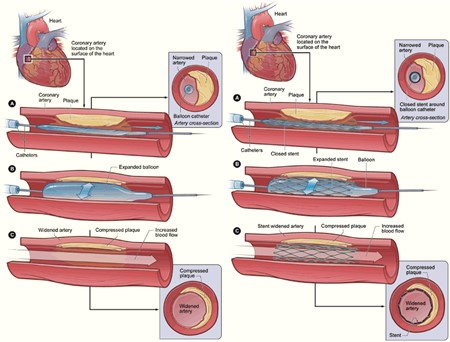
\includegraphics[scale=0.5]{./02_chaps/cap_review/figure/ballon_stent.jpg}
 \caption{Angioplastia Coronária Transluminal Percutânea com Balão inflável e Stent.}
 \label{ballon_stent}
\end{figure}

\medskip
Em 2001, \cite{hwang2001} apresenta uma simulação da implantação de um stent
revestido com uma droga em uma artéria coronária. A simulação apresentou a 
intima relação entre a distribuição da droga e o \textit{número de Peclet} 
além da importância em desenvolver geometrias para os stents que potencializem 
a difusão da substância química. Tal procedimento se mostrou uma opção promissora
para o tratamento da aterosclerose e da reestonose. Este novo tipo de stent
ficaria conhecido como \textit{stent farmacológico}.
Ao longo da década, diversos stents farmacológico foram desenvolvidos tais como:
\textit{Ravel} \cite{morice2002}, 
\textit{Taxus I e Taxus II} \cite{grube2003} \cite{colombo2003}, 
\textit{C-Sirius} \cite{schampaert2004}, 
e \textit{Smart} \cite{ardissino2004}.
